%----------------------------------------------------------
% PACKAGES AND THEMES
%----------------------------------------------------------
\documentclass[aspectratio=169,xcolor=dvipsnames,handout]{beamer}

\usetheme{Darmstadt}
\usecolortheme{seahorse}
\setbeamercovered{transparent}

\usepackage[hangul]{kotex}
\usepackage{hyperref}
\usepackage{graphicx, array, adjustbox, makecell}
\usepackage{booktabs, multicol, multirow}

% font조정
%\usepackage{fontspec}
%\setmainfont{Times New Roman}
%\setmainhangulfont{NanumGothic}

% 문자열 대체{노사관계론 전용}
\usepackage{newunicodechar}
\newunicodechar{•}{$\cdot$}
\newunicodechar{➔}{$\implies$}
\newunicodechar{∴}{$\therefore$}
\newunicodechar{∵}{$\because$}

%----------------------------------------------------------
% TITLE PAGE
%----------------------------------------------------------
\title{중대재해처벌법}
\subtitle{노사관계의 이론과 실제}
\author{오성재}
\institute[CNU]
{\relax
    충남대학교 경제학과\
    }
\date{2024년 11월 28일}

%----------------------------------------------------------
\begin{document}
%----------------------------------------------------------

\frame{\titlepage}

\begin{frame}{목차}
    \small
    \tableofcontents[hideallsubsections]
\end{frame}

\section{사실확인}%

\subsection{도입 배경}
\begin{frame}[allowframebreaks]
    \frametitle{도입 배경}
    \begin{itemize}
        \item 산업재해의 지속 발생
            \begin{itemize}
                \item 대구 지하철 화재 (2003): 192명 사망
                \item 세월호 참사 (2014): 304명 사망
                \item 태안화력발전소 사고 (2018): 노동자 사망
                \item 이천 물류창고 화재 (2020): 38명 사망
                \item 2019년 10만명당 산재 치명률은 4.6\%로 OECD 국가중 5위에 해당함 (ILO, 2021)
            \end{itemize}
    \framebreak%
        \item 사회적 요구와 캠페인
            \begin{itemize}
                \item 03년 ``산재 사망은 기업의 살인'' 캠페인 확산
                \item 14년 세월호 참사 이후, 안전 관리 강화 필요성 대두
            \end{itemize}
        \item 제도적 보완 필요
            \begin{itemize}
                \item 중대재해 기업 처벌법 재정연대 결성 (2015)
                \item 입법 청원 및 첫 입법 발의 (2017)
                \item 산업안전보건법 전면 개정 (2019) $\implies$ 20년 사고에 대한 대처 미흡.
            \end{itemize}
    \end{itemize}
\end{frame}

\subsection{주요 내용}
\begin{frame}
    \frametitle{도입과정}
    \begin{itemize}
        \item 2020년: 입법안 제출
        \item 2021년: 중대재해 처벌 등에 관한 법률 공포
        \item 2022년: 상시 근로자 50인 이상 대상 시행
        \item 2024년: 상시 근로자 5인 이상 사업장으로 확대
        \item \textbf{적용 대상:} 제조업, 건설업 등 위험도가 높은 산업군
        \item 산업안전보건법과의 차이
            \begin{itemize}[<+->]
                \item 경영진의 책임 명확화
                \item 안전·보건 조치 미이행 시 강력한 처벌
            \end{itemize}
    \end{itemize}
\end{frame}

\begin{frame}
    \frametitle{시행령 4조 (안전보건관리체계의 구축 및 이행 조치)}
        \begin{enumerate}
            \small
            \item 안전, 보건 목표와 경영방침의 설정
            \item 안전, 총괄, 관리 전담조직
            \item \textbf{유해, 위험요인 확인 개선 절차 마련 및 점검}
            \item 예산편성 및 집행
            \item 안전보건관리자에 대한 권한·예산 부여 및 \textbf{연 1회 이상 평가·관리}
            \item 안전관리자, 보건관리자 등 배치
            \item 종사자 의견청취
            \item 중대재해 대비 매뉴얼 마련 및 점검
            \item 제3자에 대한 도급 관련 기준과 절차 마련 및 점검
        \end{enumerate}
\end{frame}

\section{판결}
\begin{frame}
    \frametitle{사건 관련 통계}
    \begin{itemize}[<+->]
        \item 23년 12월 현재 중처법 대상사건은 510건 (이재현, 2024)
            \begin{itemize}[<+->]
                \item 검찰송치 170여건
                \item 내사종결 50여건
                \item 고용노동부 수사진행 290건
            \end{itemize}
        \item 24년 10월 현재 1심판결은 총 25건 (김광수, 2024)
        \end{itemize}
\end{frame}

\begin{frame}[allowframebreaks]
    \frametitle{판결결과}
    \centering
    \begin{figure}
        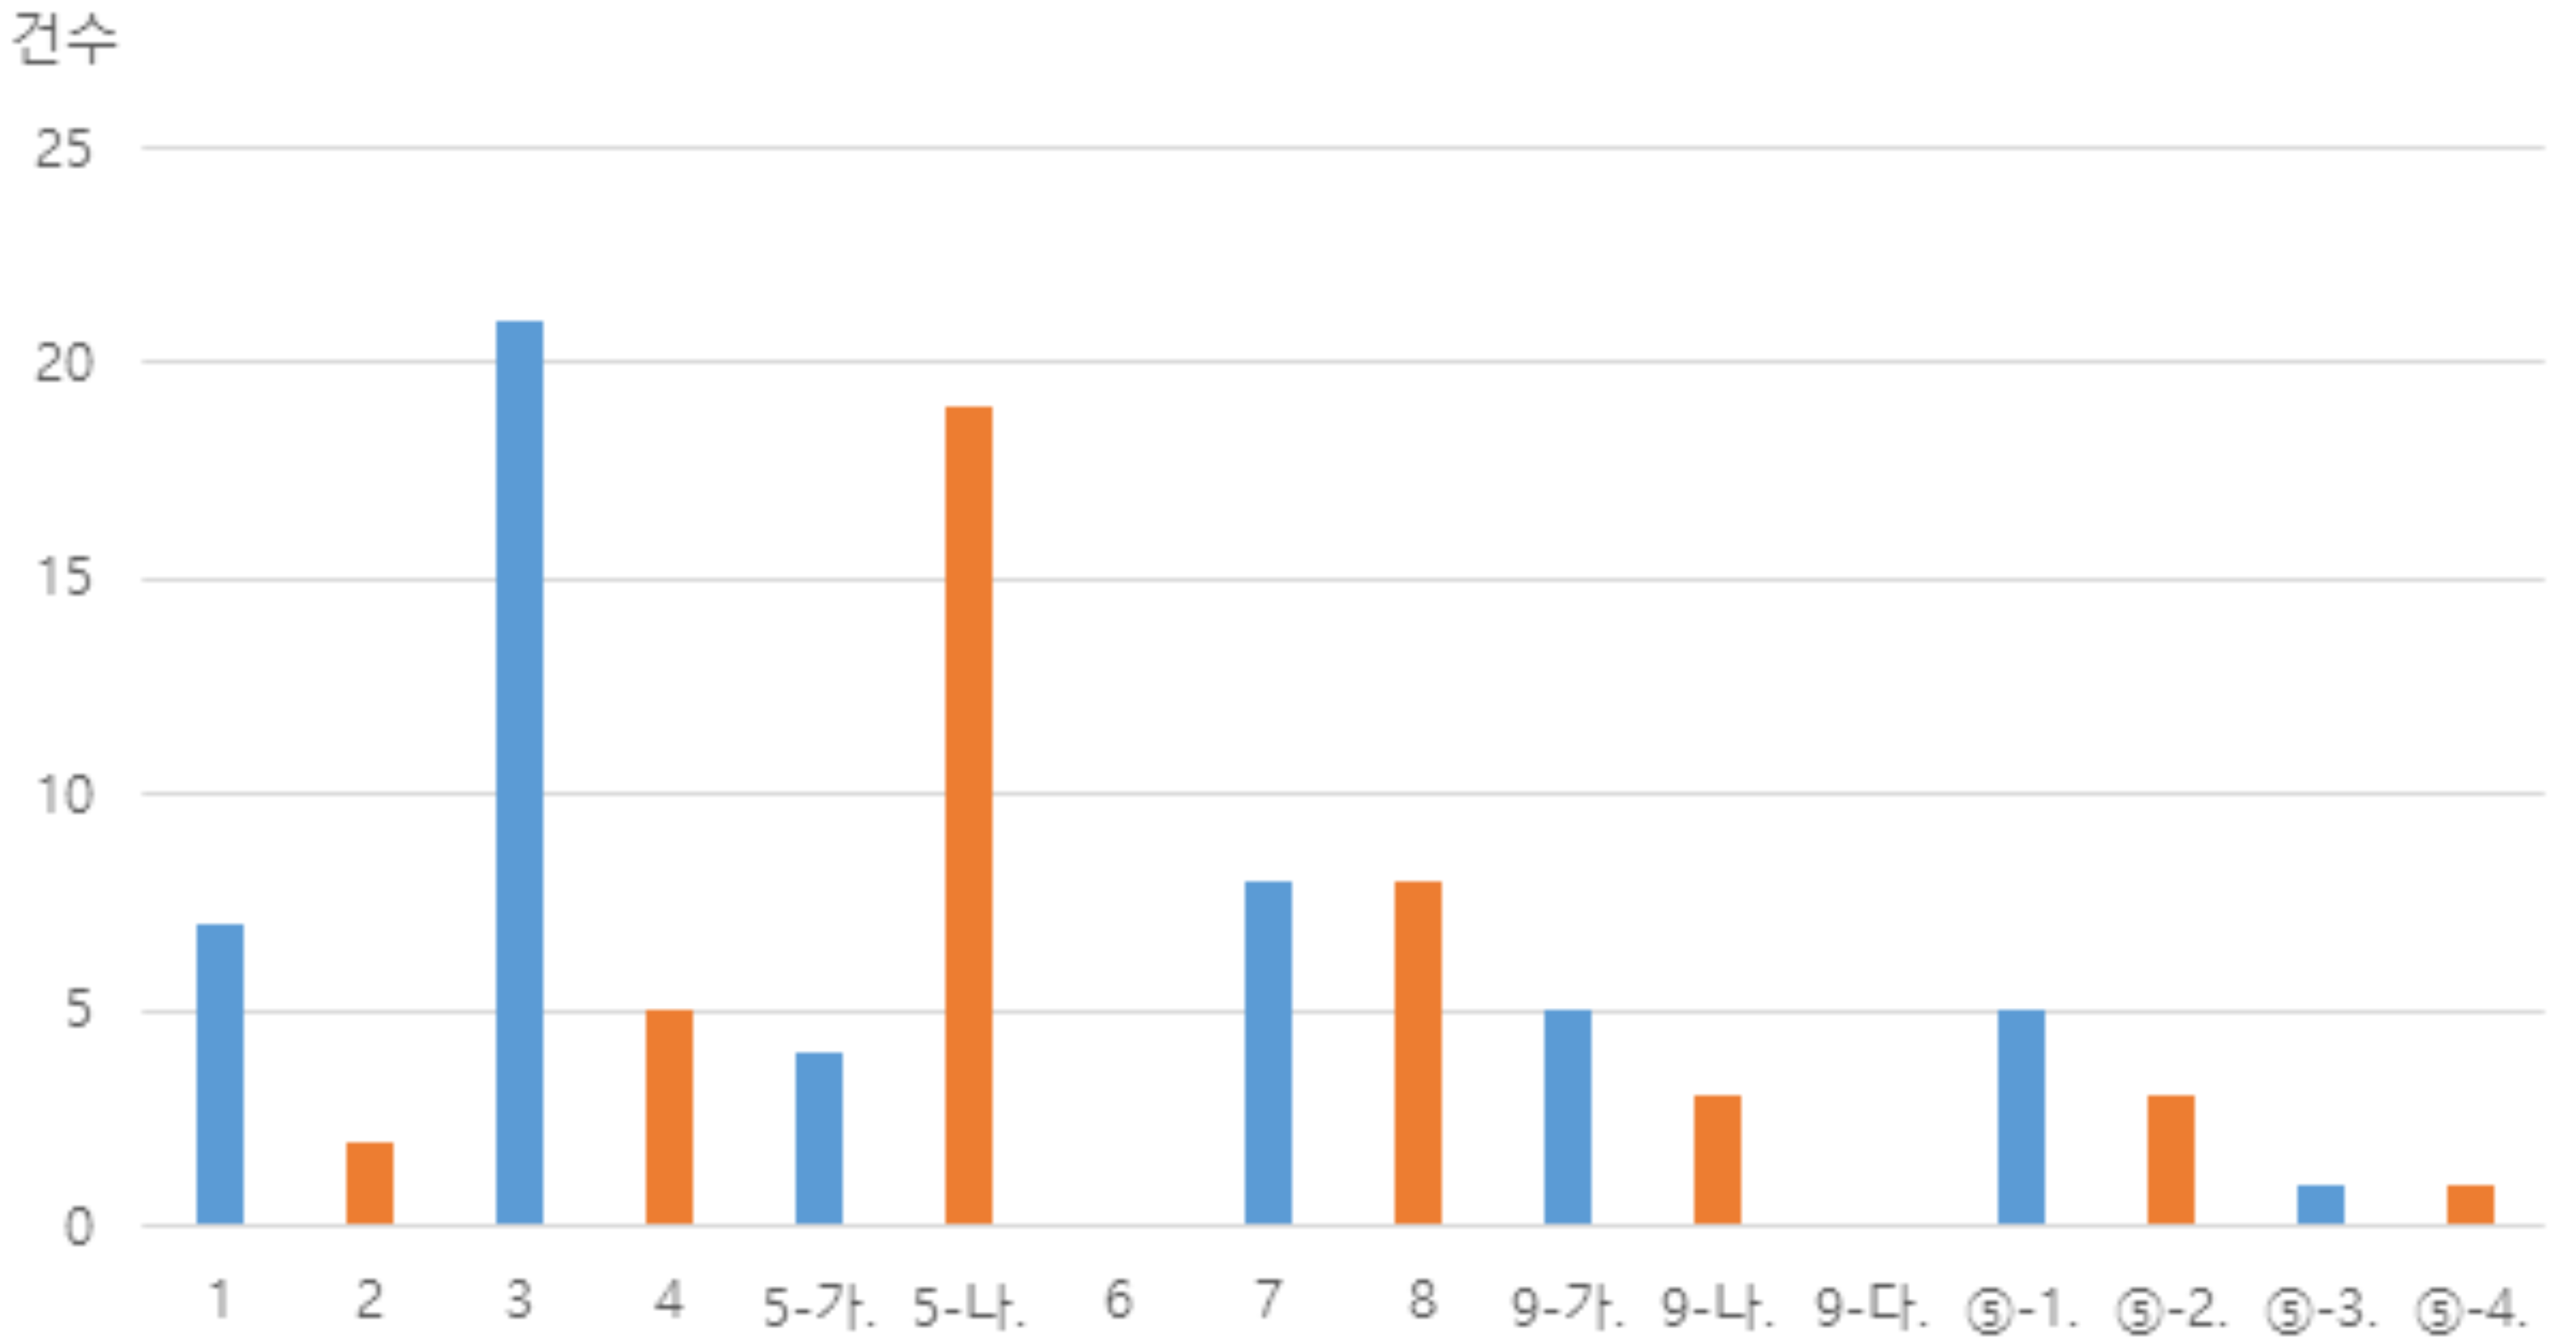
\includegraphics[width=.6\textwidth]{pic/판결의무기준}
        \\
        \raggedright%
        \hspace{1em}
        \tiny{자료: 김광수 (2024)} 
        \caption{판결의 안전·보건 확보의무 위반 현황}
    \end{figure}
\framebreak%
    \centering
    \begin{figure}
        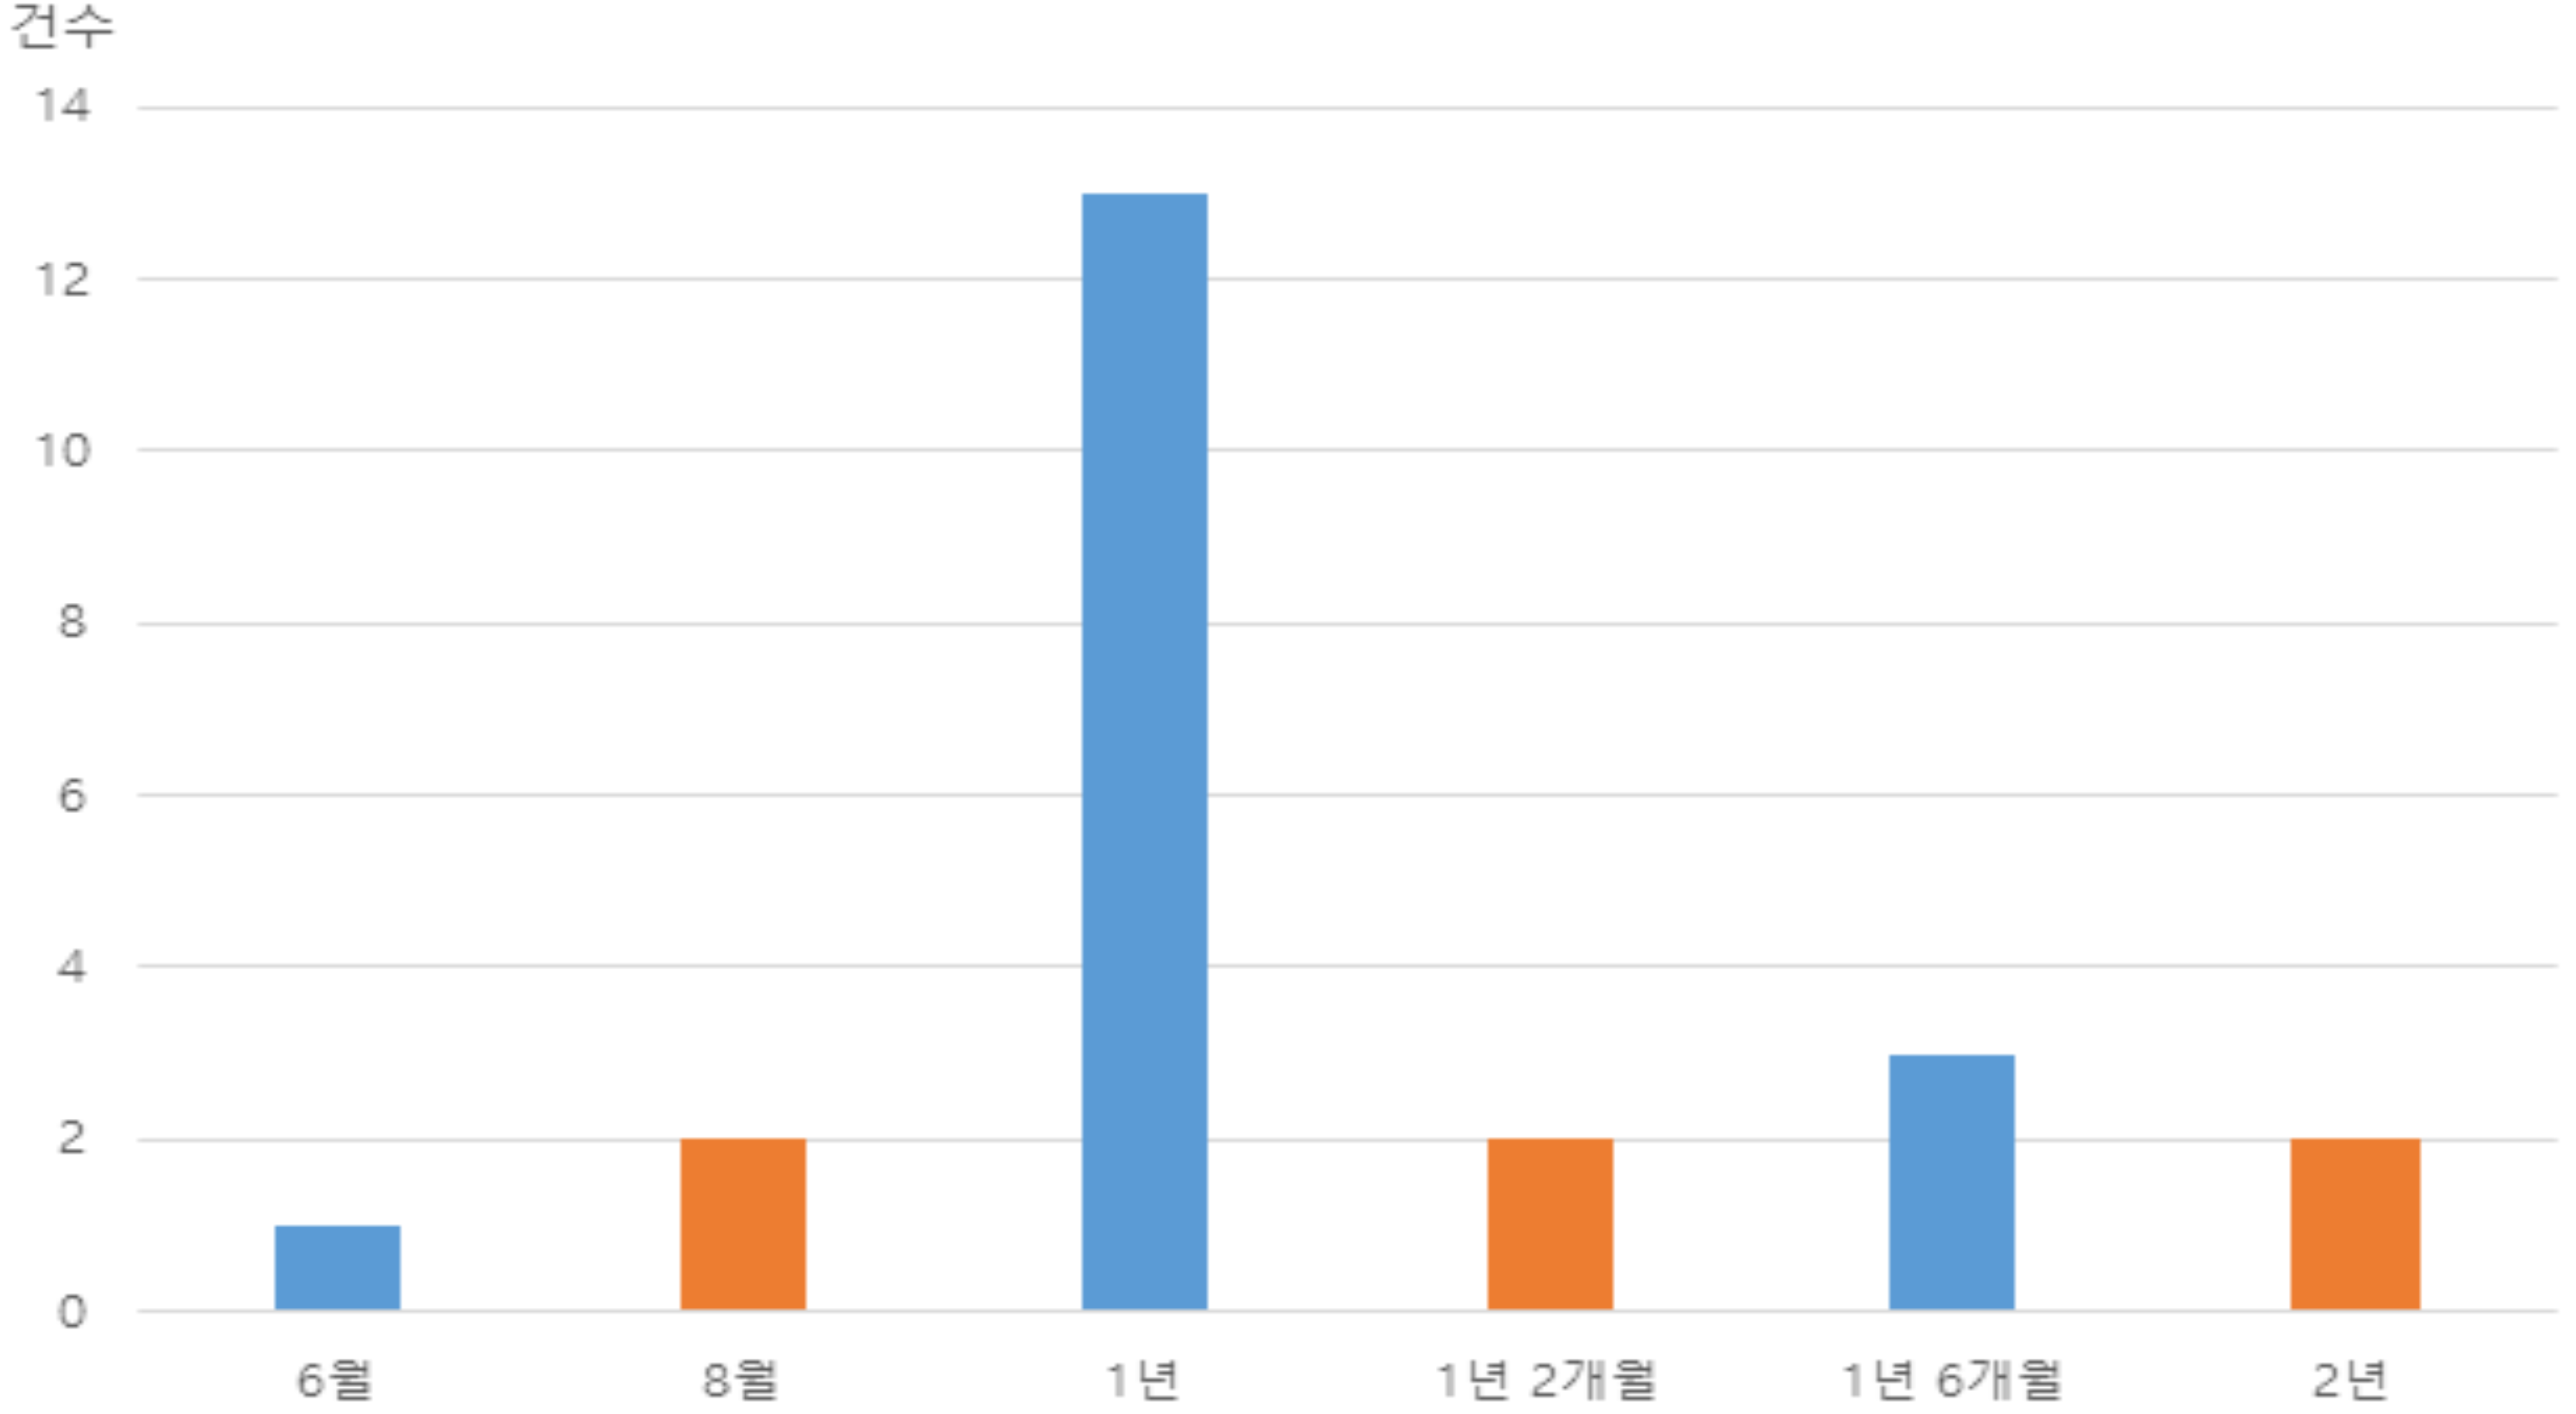
\includegraphics[width=.6\textwidth]{pic/경영책임자징역형}
        \\
        \raggedright%
        \hspace{1em}
        \tiny{자료: 김광수 (2024)} 
        \caption{경영책임자에 대한 징역형 선고 현황}
    \end{figure}
\framebreak%
    \centering
    \begin{figure}
        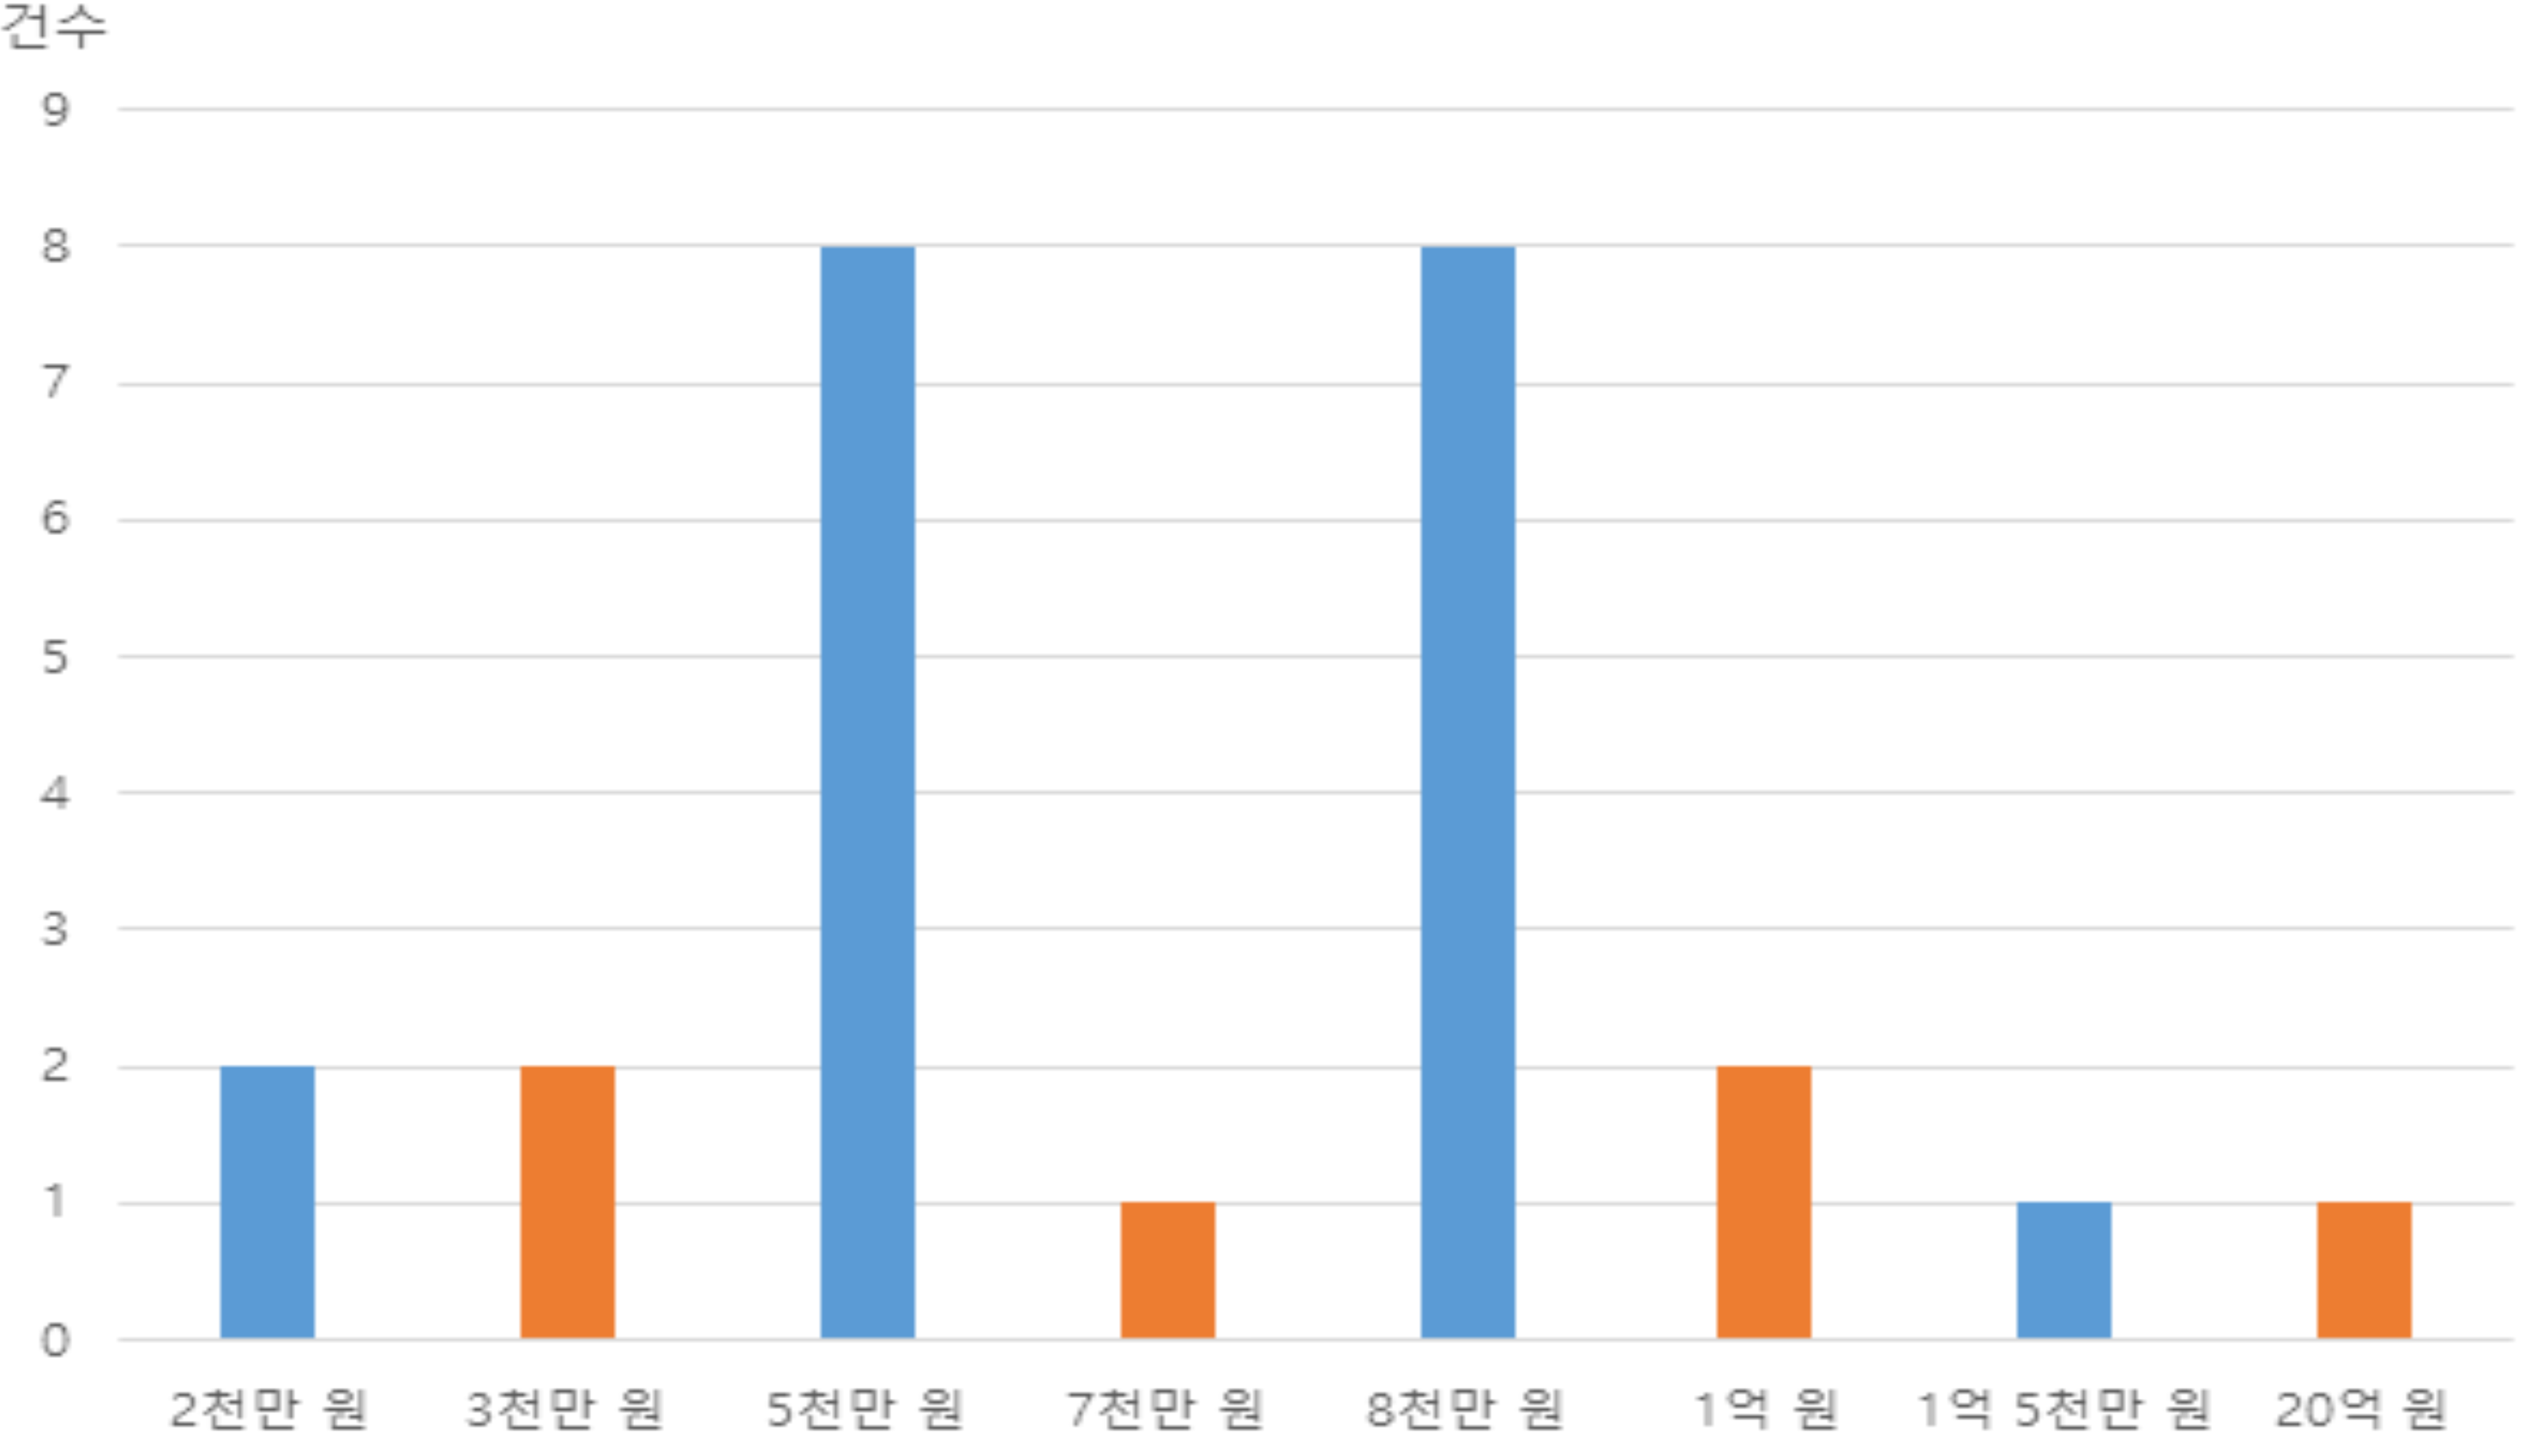
\includegraphics[width=.6\textwidth]{pic/법인벌금형}
        \\
        \raggedright%
        \hspace{1em}
        \tiny{자료: 김광수 (2024)} 
        \caption{법인에 대한 벌금형 선고 현황}
    \end{figure}
\end{frame}

\section{법의 효과}
\begin{frame}
    \frametitle{김소연 외. (2024)}
    \begin{itemize}[<+->]
        \item 고용노동부 중대 재해 발생사업장 자료와 주식시장 자료를 이용한 실증분석 연구
        \item 2009년부터 2020년까지 한 번이라도 중대 재해가 발생한 기업의 경우,
\begin{itemize}
               \item 무재해 기업과 비교하여 중대재해처벌법 통과 시점에 유의한 음 (-)의 비정상 수익률을 기록
               \item 중대 재해 발생 횟수가 많을수록 주가가 더 크게 하락
        \item 주식 시장 에서 중대 재해 발생 이력이 있는 기업에 대해 중대재해처벌법으로 향후 손실이 발생할 가능성이 더 높다고 평가
\end{itemize}
        \item 한편, 기업의 ESG 등급 및 E, S, G 개별 등급이 좋을수록 중대 재해 발생 기업의 주가 하락이 완화
\begin{itemize}
               \item ESG 성과가 중대재해처벌법에 의한 위험을 감소
\end{itemize}
    \end{itemize}
\end{frame}

\begin{frame}
    \frametitle{박재옥 and 한순구 (2024)}
    \begin{itemize}[<+->]
        \item 게임이론적 분석: 사업주와 근로자의 손익과 주의력
        \item 사업주와 경영책임자의 책임을 강화하는것 만으로는 사고가 줄어 든다는 보장이 없음
\begin{itemize}
               \item 발생건수 역시 사고 및 재해의 유의한 감소는 없음
               \item 사업자의 근로자에 대한 통제력이 충분하지 않음 $\implies$ 근로자들이 법 시행후 안전에 대한 주의를 낮출 가능성.
               \item 통제가 쉬운 제조업에서는 사망사고 감소. 반면, 건설업에서는 오히려 증가
\end{itemize}
        \item 법의 사고발생 및 사회적 후생에 미치는 영향을 분석하기 위해서는 사업주와 경영책임자의 근로자에 대한 통제력이 함께 고려되어야
    \end{itemize}
\end{frame}


\section{시사점}
\begin{frame}
    \frametitle{이재현 (2024)}
    \centering
    \begin{figure}
        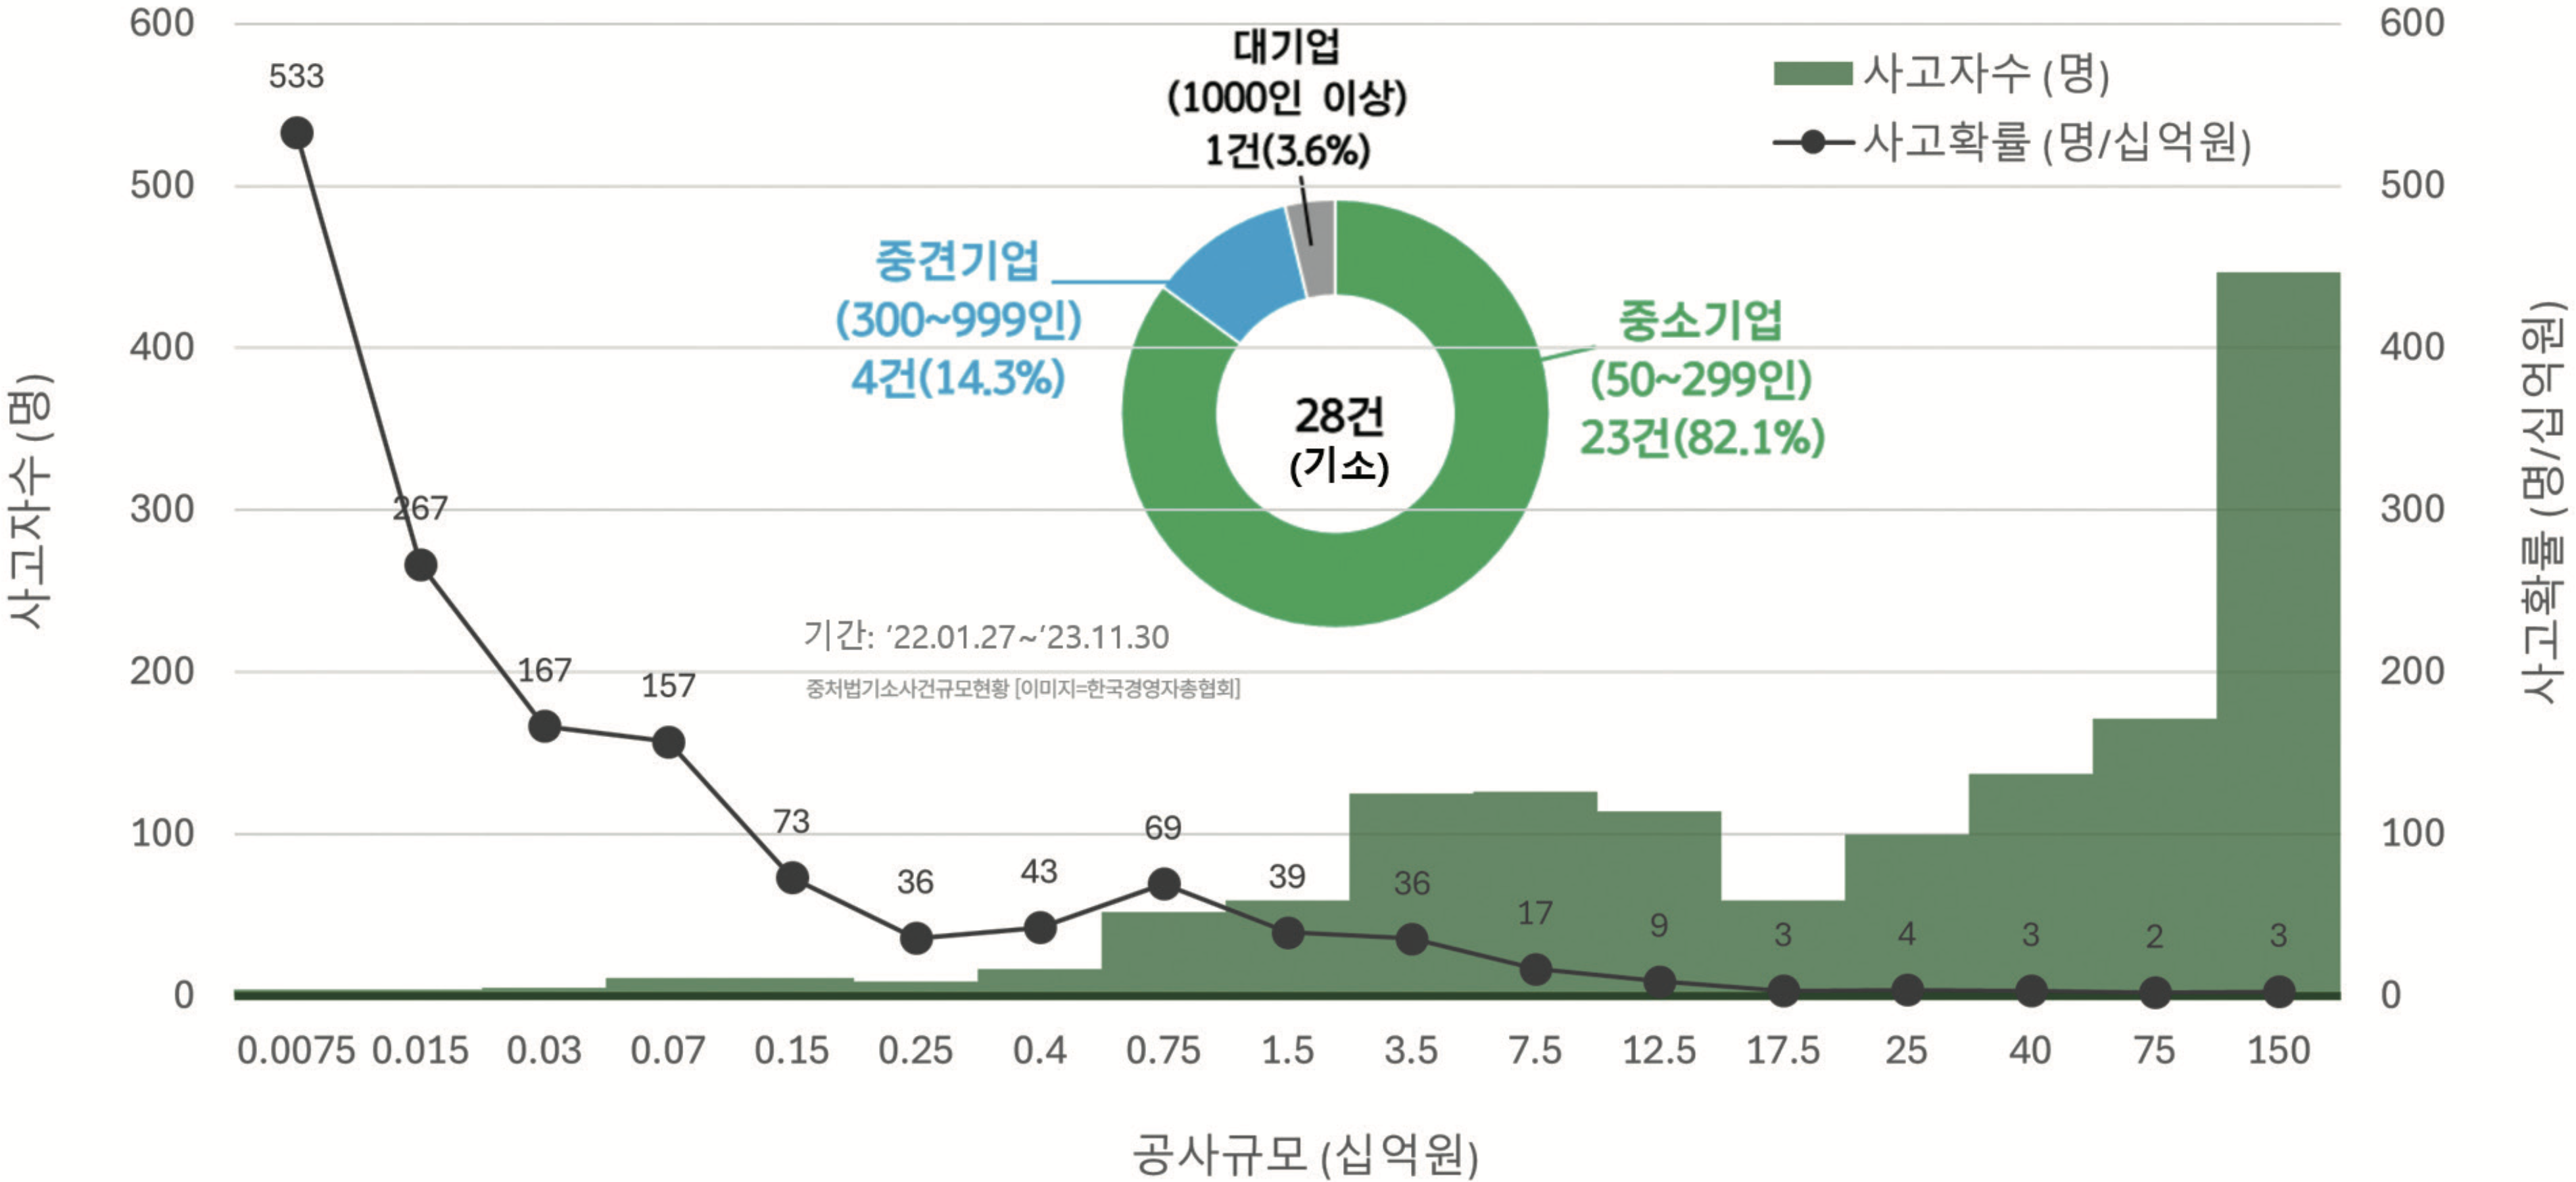
\includegraphics[width=.8\textwidth]{pic/공사규모별사고자수및확률}
        \\
        \raggedright%
        \hspace{1em}
        \tiny{자료: 이재현 (2024)}
        \caption{공사규모별 사고자수 및 사고확률}
    \end{figure}
\end{frame}

\begin{frame}
    \frametitle{김광수 (2024)}
    \begin{itemize}[<+->]
        \item 기존법 (산업안전보건법)과 중첩
        \item 핵심내용을 법률이 아닌 시행령에 규정
        \begin{itemize}
            \item 시행령 상 의무를 중대재해처벌법으로 편입해야
        \end{itemize}
        \item 재해라는 결과가 발생한 경우에만 처벌 
        \begin{itemize}
            \item 의무 위반 규제 및 처벌을 통해 중대재해에 대한 선제적·효과적인 대응
        \end{itemize}
    \end{itemize}
\end{frame}

\section*{참고문헌}
\begin{frame}
    \frametitle{참고문헌}
    \begin{itemize}[<+->]
        \item 김광수. (2024). 중대재해처벌법의 적용에 관한 연구 -하급심 판결의 분석을 중심으로-. 형사정책, 36(3), 159--210.
        \item 김소연, 박세열 and 박순홍. (2024). 중대재해처벌법 제정의 공시 효과 분석. 기업과혁신연구, 47(3), 89--106.
        \item 박재옥 and 한순구. (2024). 중대재해처벌법은 재해를 감소할 수 있는가?. 한국경제포럼, 16(4), 1--28.
        \item 이재현. (2024). 중대재해처벌법 판례 및 시사점. 건축시공, 24(3), 5--10.
    \end{itemize}
\end{frame}

%------------------------------------------------
\end{document}
%------------------------------------------------

